\subsection{Results}\label{Testing:Results}
	In this section we will go over the results for each of the test cases in the preceding section. We will compare the results with each other and also compare most of the cases to the "No throttle mediator" scenario.
	
	\begin{shaded}
	To see all the results of our tests in their raw forms, we refer you to appendix \ref{RawResults}.
	\end{shaded}
	 
    \textbf{Test case 1:}\\
    In test 1 we wanted to find out how the ESB would perform with a low timeout. From our expectations we want to see that the average time for messages to arrive is low, but we do not expect this test to have as good a percentage as the rest. 
    
	\begin{figure}[H]
		\centering
		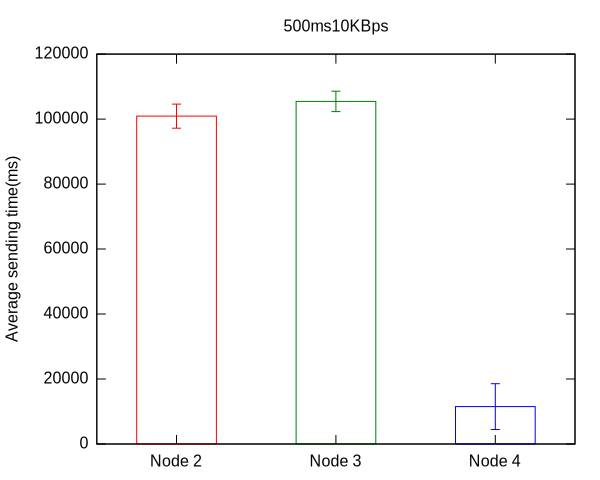
\includegraphics[scale=0.5]{500ms10KBps_time}
		\caption{Time graph, timeout equal to 500 and bandwidth of 10kBps} 
		\label{figure:results:500ms10KBps_time}
	\end{figure}
	
	\begin{figure}[H]
		\centering
		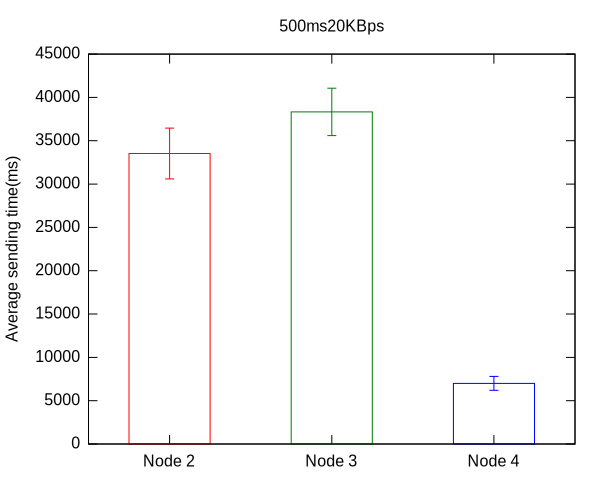
\includegraphics[scale=0.5]{500ms20KBps_time}
		\caption{Time graph, timeout equal to 500 and bandwidth of 20kBps} 
		\label{figure:results:500ms20KBps_time}
	\end{figure}
    
    The actual results do indeed match our expectation quite well. As you can see in figure \ref{figure:results:500ms20KBps_time} the time taken is quite low, if we compare that time to the time in figure \ref{figure:results:2000ms20KBps_time} we can easily see that the lower timeout has an effect on the results and in most of the cases it is correct that the lower timeout does make the ESB quicker.
    
    \begin{figure}[H]
		\centering
		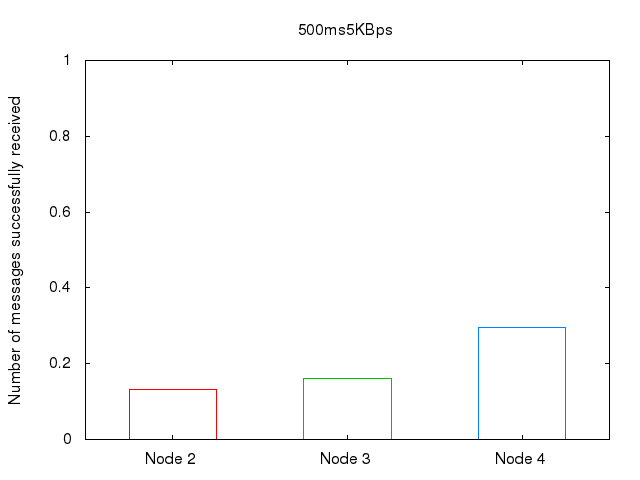
\includegraphics[scale=0.5]{500ms5KBps_messages}
		\caption{Message graph, timeout equal to 500 and bandwidth of 5kBps} 
		\label{figure:results:500ms5KBps_messages}
	\end{figure}
	
	As a last piece of result we have added the message graph with a bandwidth of 5kBps which should give a glimpse into how increasing the timeout effects the number successful messages received.
    
    \textbf{Test case 2:}\\
    As we stated in the section \ref{Testing:Cases} we expect this setting to do a bit better than with a timeout of 500ms when it comes to number of successful messages.
    \begin{figure}[H]
		\centering
		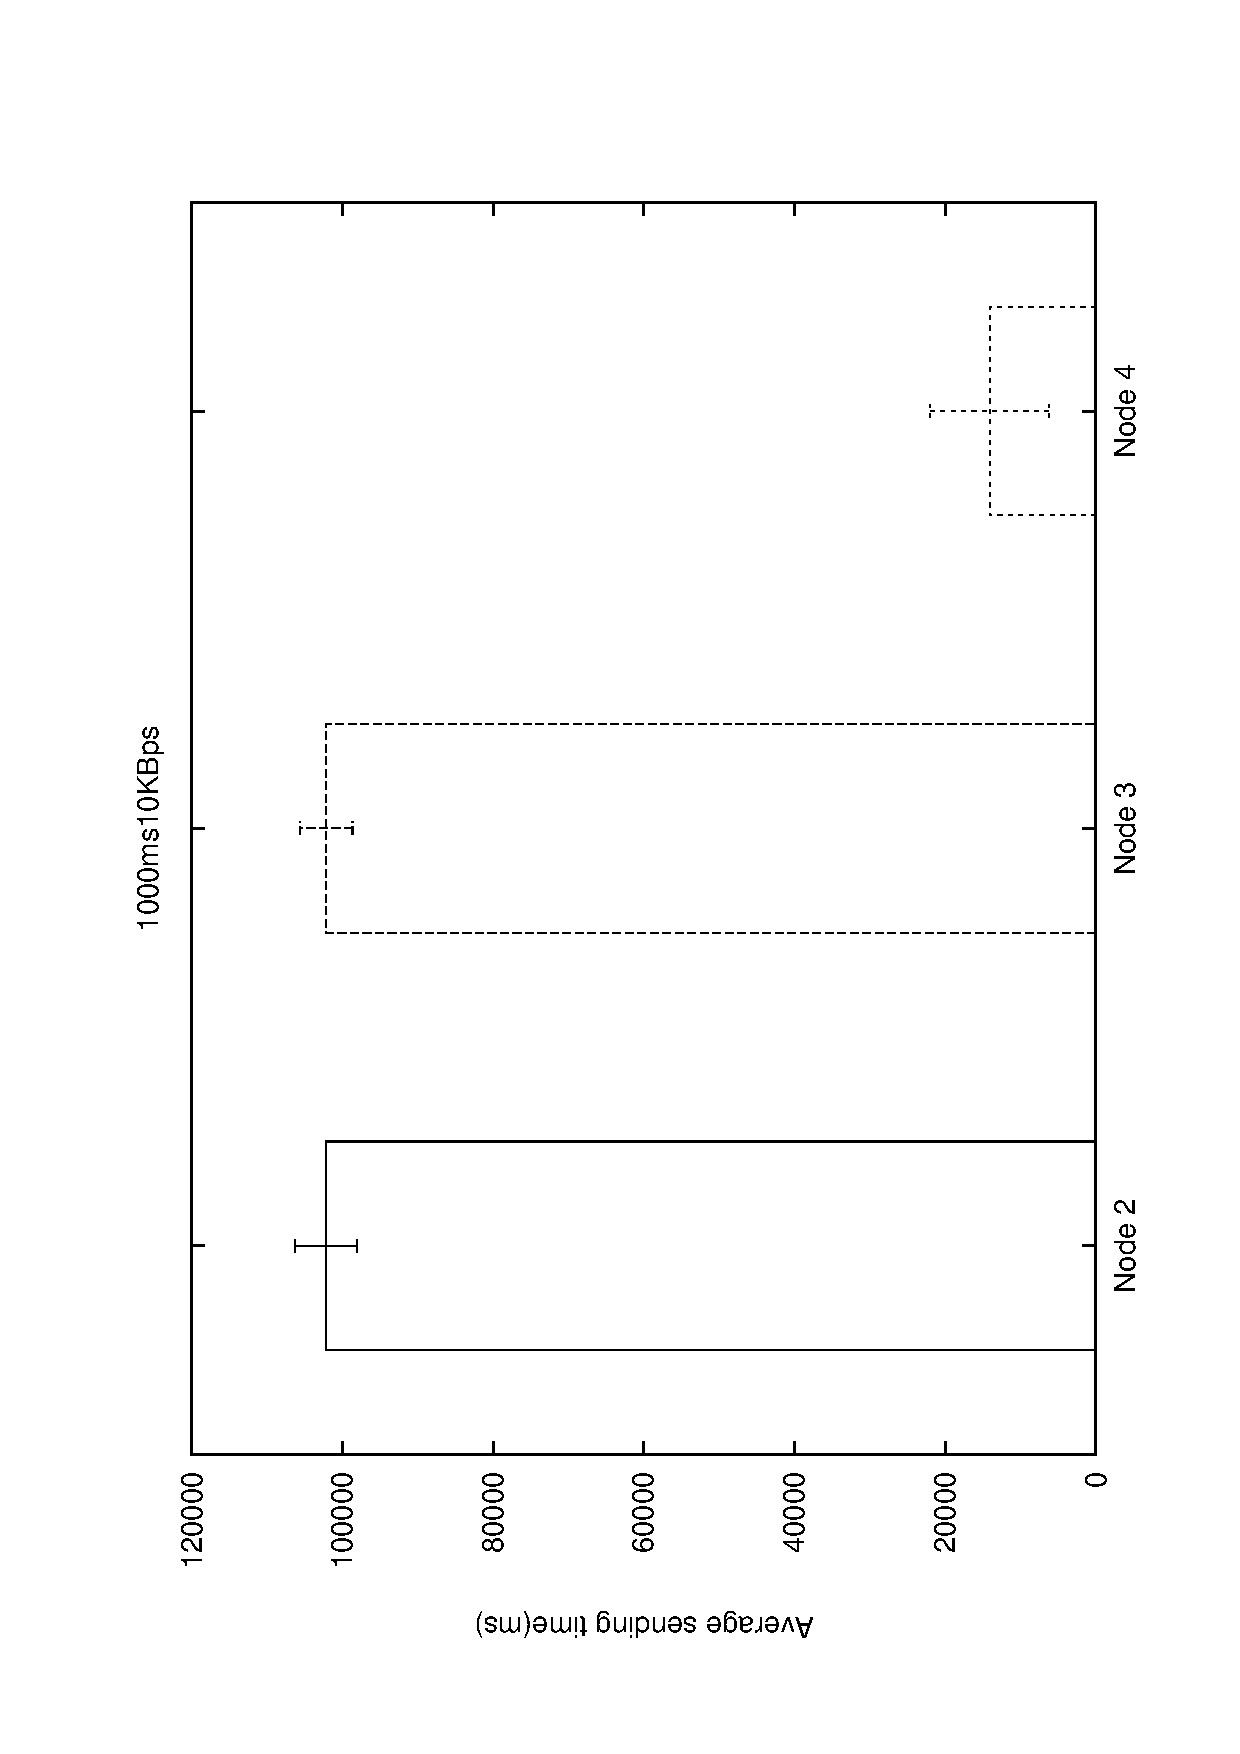
\includegraphics[scale=0.5]{1000ms10KBps_time}
		\caption{Time graph, timeout equal to 1000 and bandwidth of 10kBps} 
		\label{figure:results:1000ms10KBps_time}
	\end{figure}
	
	\begin{figure}[H]
		\centering
		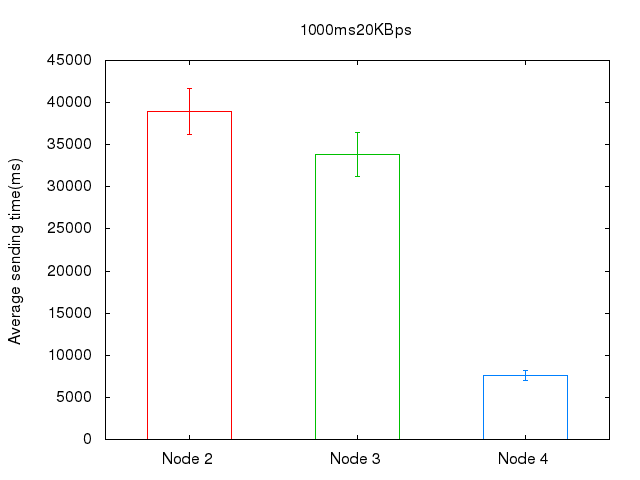
\includegraphics[scale=0.5]{1000ms20KBps_time}
		\caption{Time graph, timeout equal to 1000 and bandwidth of 20kBps} 
		\label{figure:results:1000ms20KBps_time}
	\end{figure}
	
	From the figures it might not be clear, but the results are actually not what we expected. The test is better with regard to successful messages with a timeout of 500ms than on 1000ms and the time taken is within the standard deviation so we can't say much about that either.
	
	\begin{figure}[H]
		\centering
		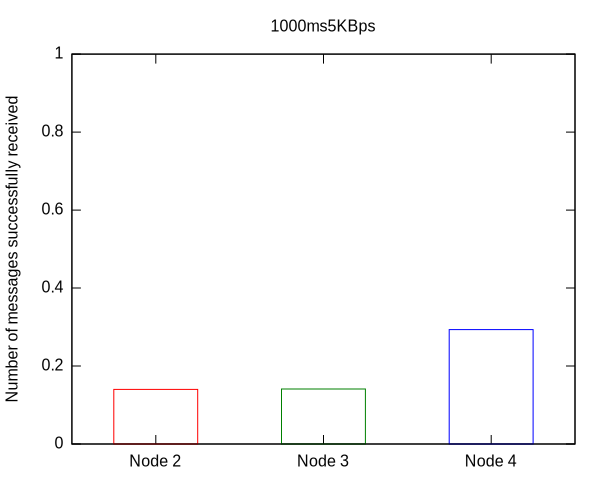
\includegraphics[scale=0.5]{1000ms5KBps_messages}
		\caption{Message graph, timeout equal to 1000 and bandwidth of 5kBps} 
		\label{figure:results:1000ms5KBps_messages}
	\end{figure}
	
	The history here is the same as with 500ms timeout.
    
    \textbf{Test case 3:}\\
    We expected this test to have some increase in successful messages compared to the two previous results. The average time taken should however drop slightly.
    \begin{figure}[H]
		\centering
		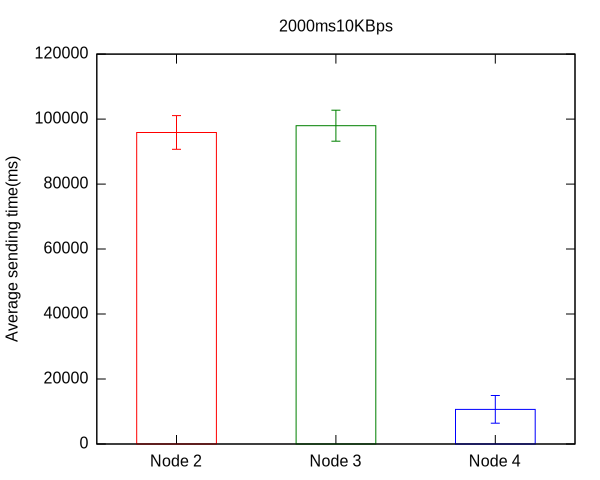
\includegraphics[scale=0.5]{2000ms10KBps_time}
		\caption{Time graph, timeout equal to 2000 and bandwidth of 10kBps} 
		\label{figure:results:2000ms10KBps_time}
	\end{figure}
	
	\begin{figure}[H]
		\centering
		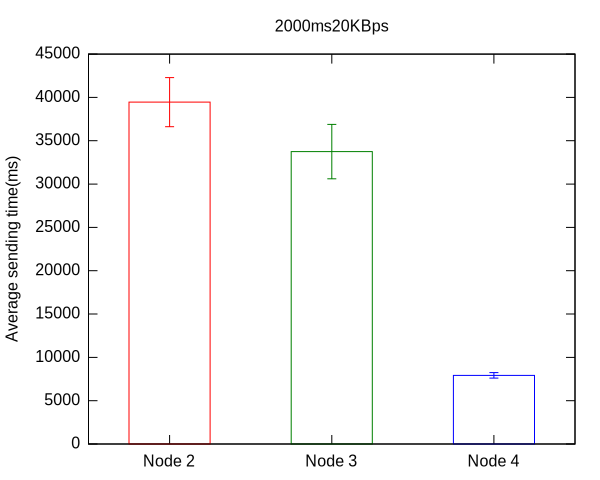
\includegraphics[scale=0.5]{2000ms20KBps_time}
		\caption{Time graph, timeout equal to 2000 and bandwidth of 20kBps} 
		\label{figure:results:2000ms20KBps_time}
	\end{figure}
	
	The result we got for this test also surprised us a bit. The number of successful messages has increased with quite a bit compared to a timeout of 500ms. Which is what we expected, but with result of 1000ms this might not have been the case. What is really strange is that the average time has dropped.
	
	\begin{figure}[H]
		\centering
		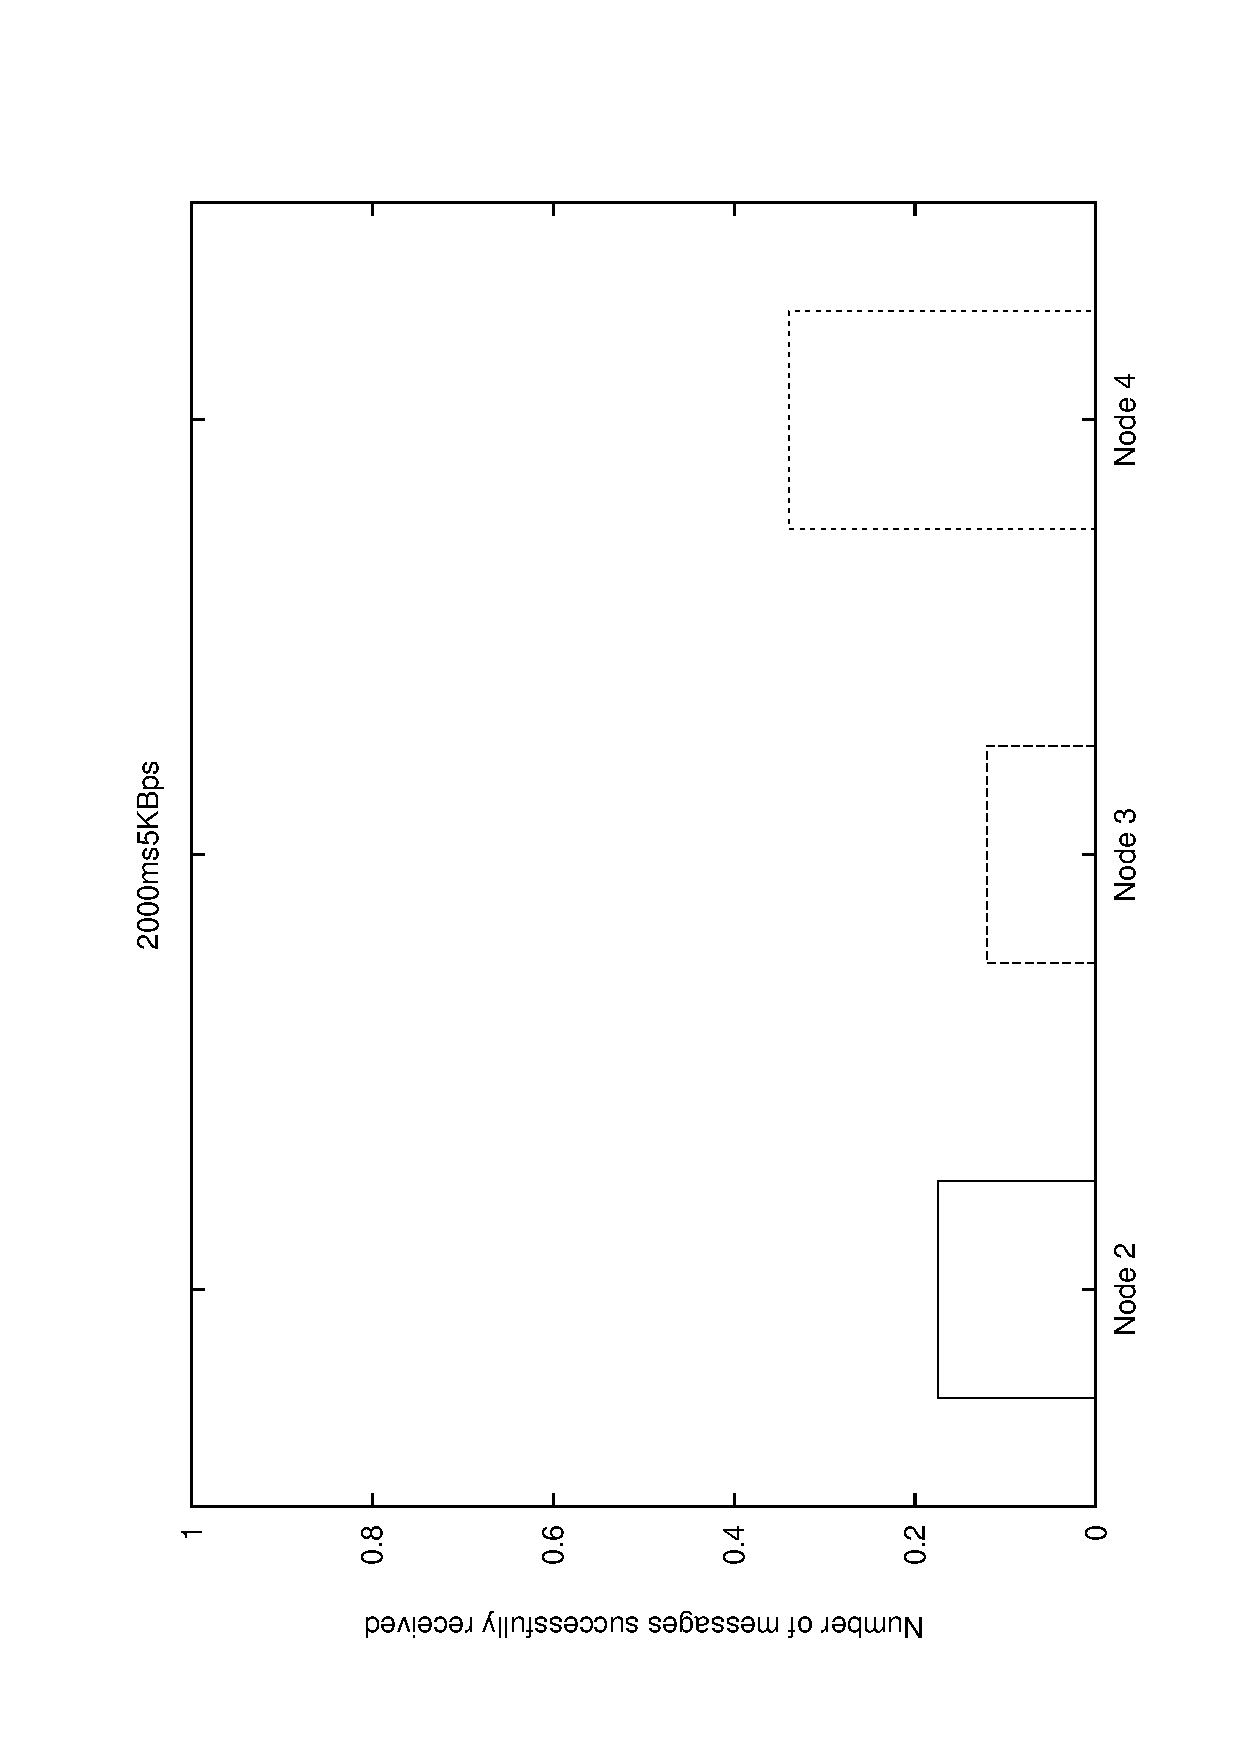
\includegraphics[scale=0.5]{2000ms5KBps_messages}
		\caption{Message graph, timeout equal to 2000 and bandwidth of 5kBps} 
		\label{figure:results:2000ms5KBps_messages}
	\end{figure}
    Here the result is a bit brighter than before, and we can see that more messages arrive because of the increased timeout.
    
    \textbf{Test case 4:}\\
    We expected more messages to arrive here compared to the previous tests.
    \begin{figure}[H]
		\centering
		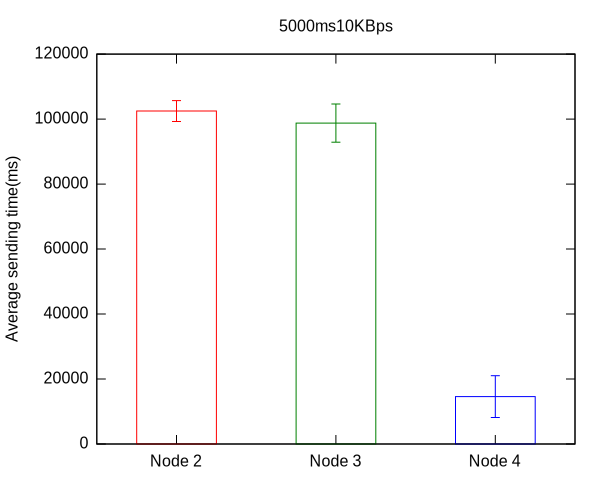
\includegraphics[scale=0.5]{5000ms10KBps_time}
		\caption{Time graph, timeout equal to 5000 and bandwidth of 10kBps} 
		\label{figure:results:5000ms10KBps_time}
	\end{figure}
	
	\begin{figure}[H]
		\centering
		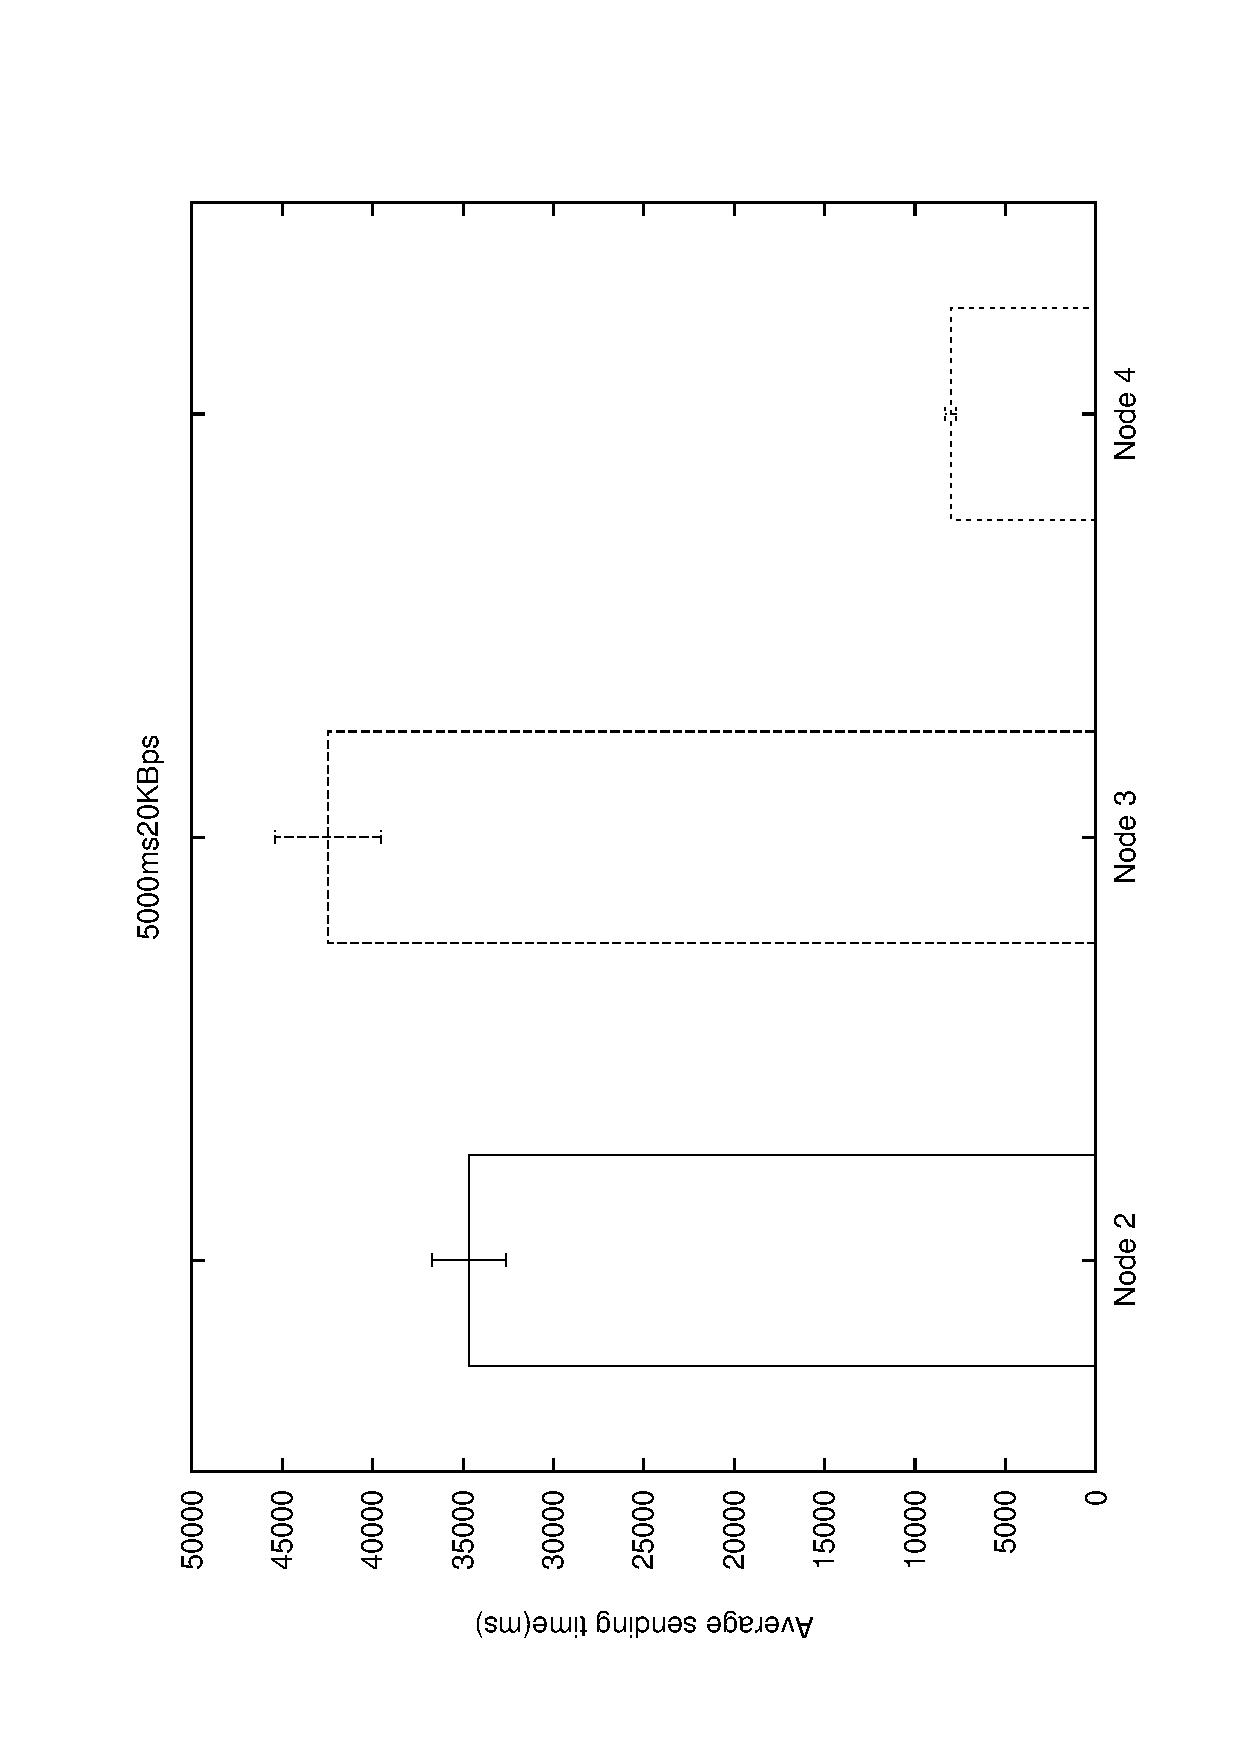
\includegraphics[scale=0.5]{5000ms20KBps_time}
		\caption{Time graph, timeout equal to 5000 and bandwidth of 20kBps} 
		\label{figure:results:5000ms20KBps_time}
	\end{figure}
	
	The story is not very different from what we expected. On average more messages arrive successfully compared to the previous three test cases. The time has also increased slightly, but is again within the standard deviation on most bandwidths.
	
	\begin{figure}[H]
		\centering
		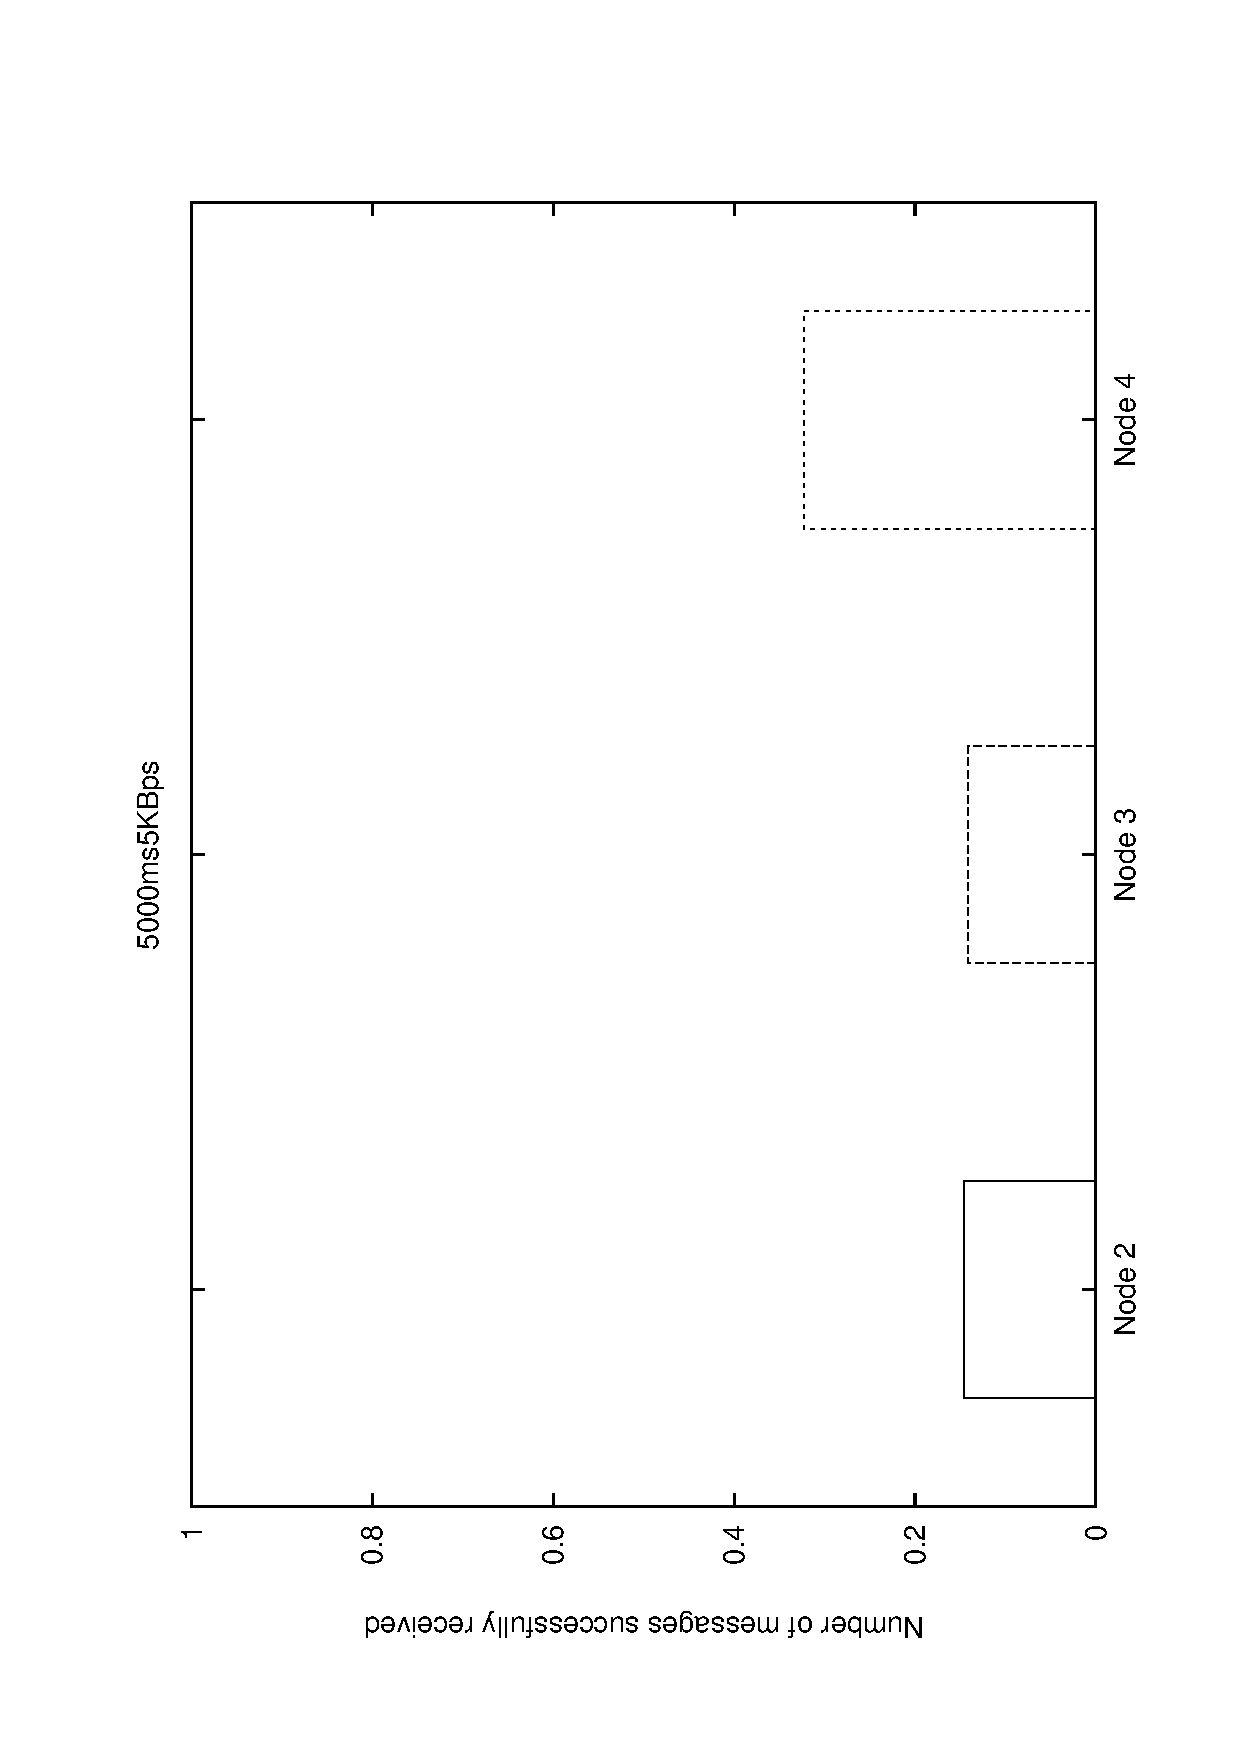
\includegraphics[scale=0.5]{5000ms5KBps_messages}
		\caption{Message graph, timeout equal to 5000 and bandwidth of 5kBps} 
		\label{figure:results:5000ms5KBps_messages}
	\end{figure}
	The results for successful messages on 5kBps is very similar to the 2000ms results, but is better than the first two tests.
    
    \textbf{Test case 5:}\\
    In this test we wanted to see how the ESB behaved with a large timeout.
    \begin{figure}[H]
		\centering
		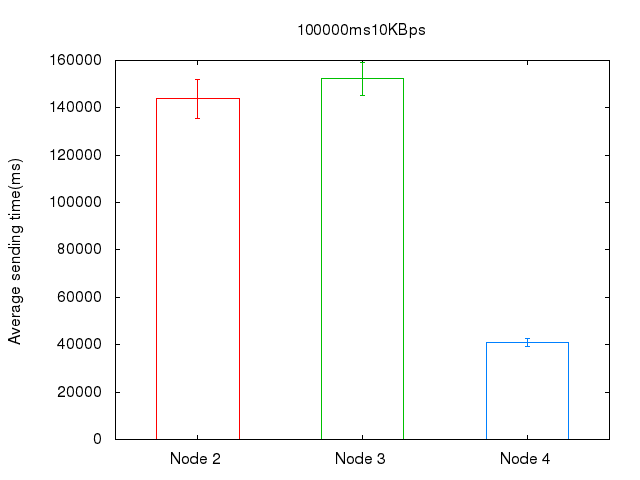
\includegraphics[scale=0.5]{100000ms10KBps_time}
		\caption{Time graph, timeout equal to 100000 and bandwidth of 10kBps} 
		\label{figure:results:100000ms10KBps_time}
	\end{figure}
	
	\begin{figure}[H]
		\centering
		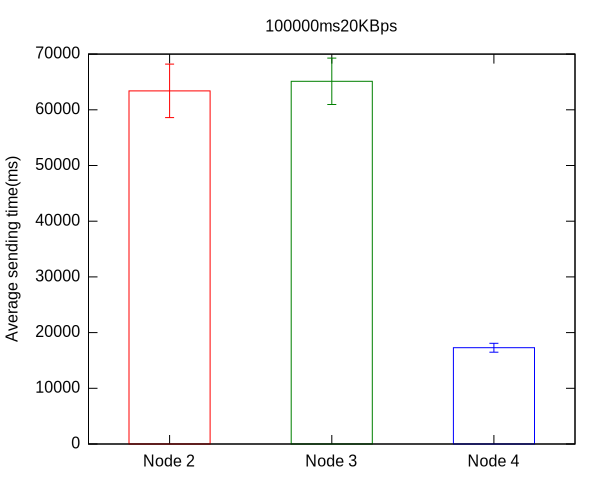
\includegraphics[scale=0.5]{100000ms20KBps_time}
		\caption{Time graph, timeout equal to 100000 and bandwidth of 20kBps} 
		\label{figure:results:100000ms20KBps_time}
	\end{figure}
	
	As we expected with such a large timeout more messages arrive successfully compared to the previous tests. The time has dramatically increased which is a direct result of the higher number of successful messages. The few deviations that we see are most likely due to random fluctuations in the test suite. 
	
	\begin{figure}[H]
		\centering
		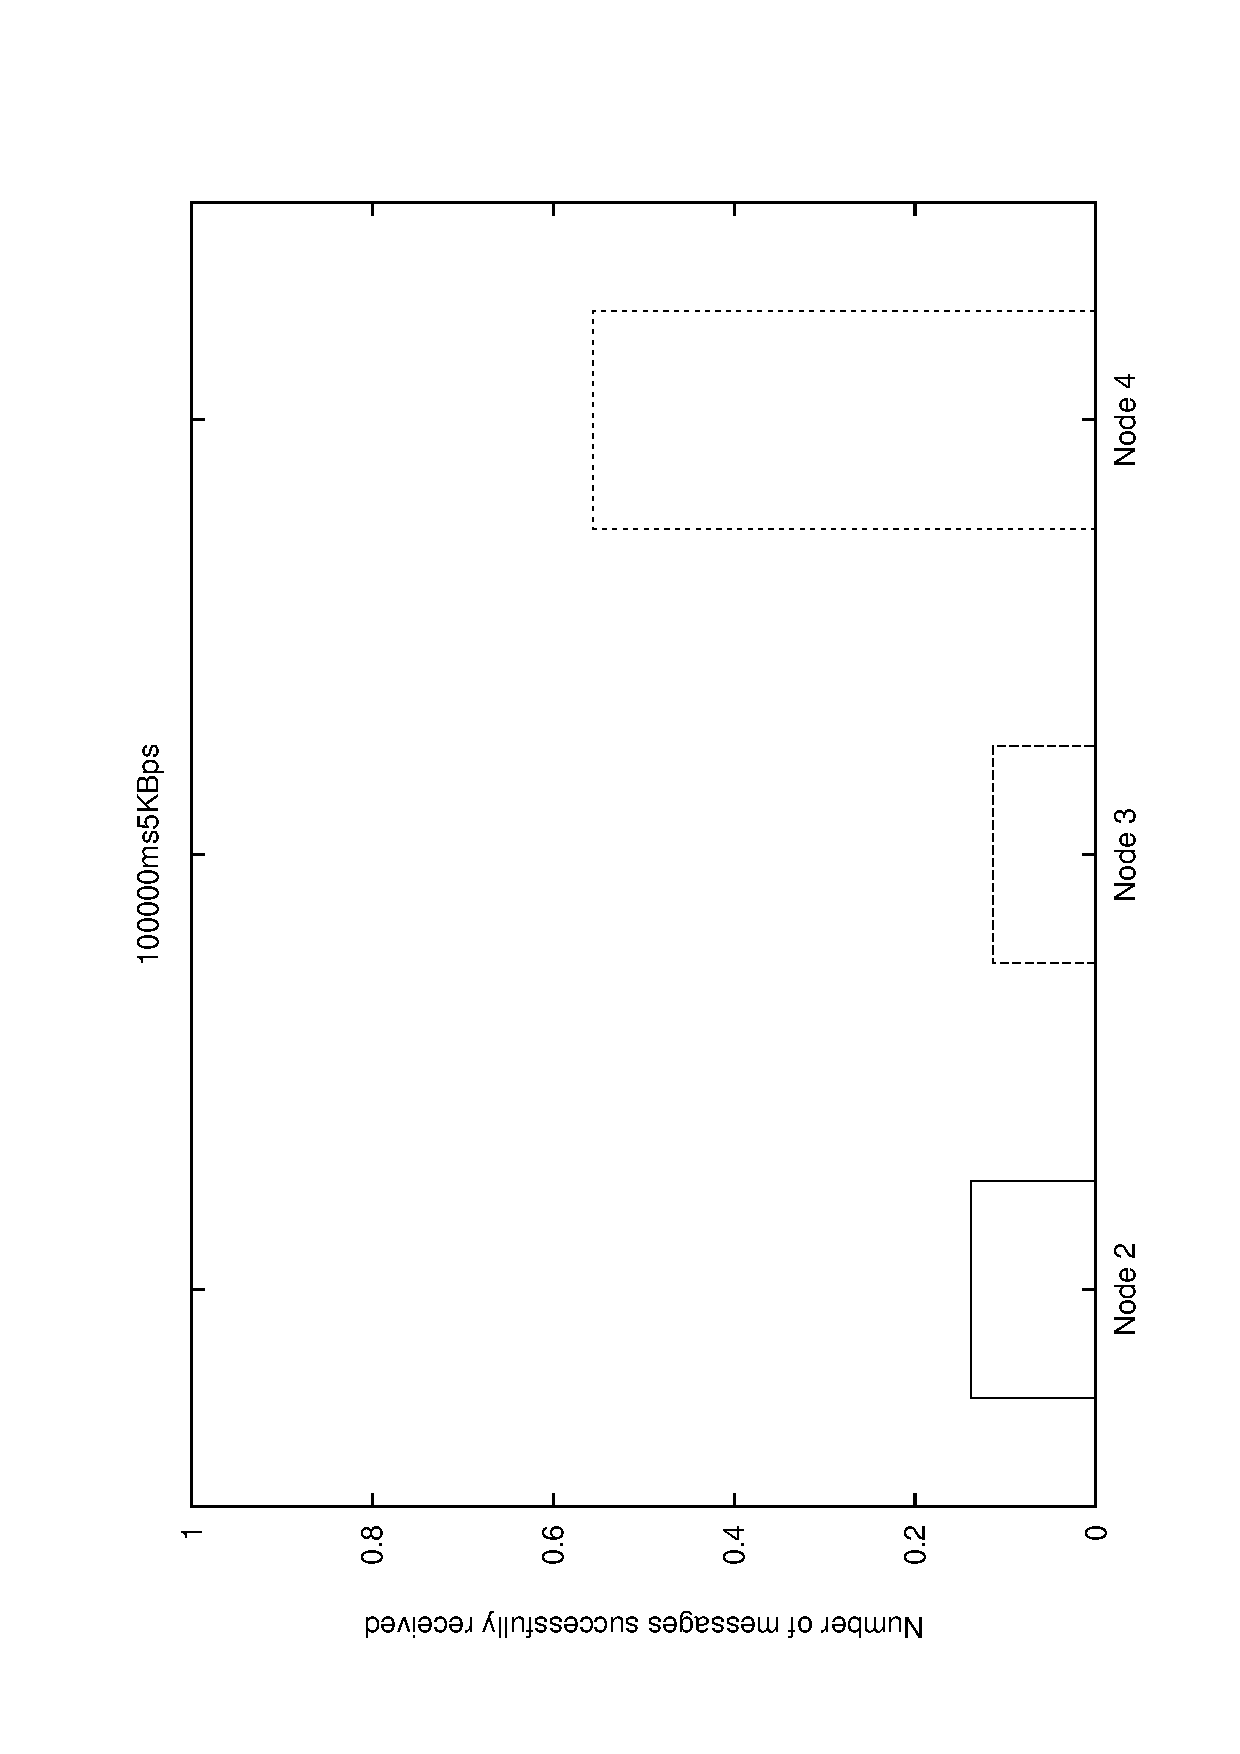
\includegraphics[scale=0.5]{100000ms5KBps_messages}
		\caption{Message graph, timeout equal to 100000 and bandwidth of 5kBps} 
		\label{figure:results:100000ms5KBps_messages}
	\end{figure}
	As with the previous test we can see an increased again, which is due to the timeout.
    
    \textbf{Test case 6:}\\
    Without the throttle mediator we expect that the results below is better with regard to number of successful messages, but worse with regard to time.
    \begin{figure}[H]
		\centering
		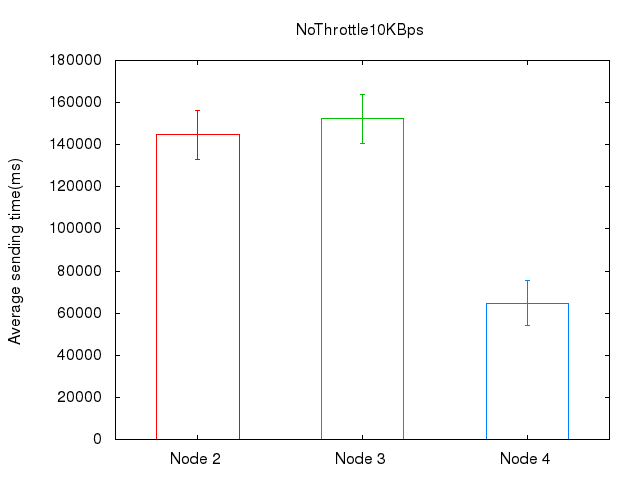
\includegraphics[scale=0.5]{NoThrottle10KBps_time}
		\caption{Time graph, no throttle mediator and bandwidth of 10kBps} 
		\label{figure:results:NoThrottle10KBps_time}
	\end{figure}
	
	\begin{figure}[H]
		\centering
		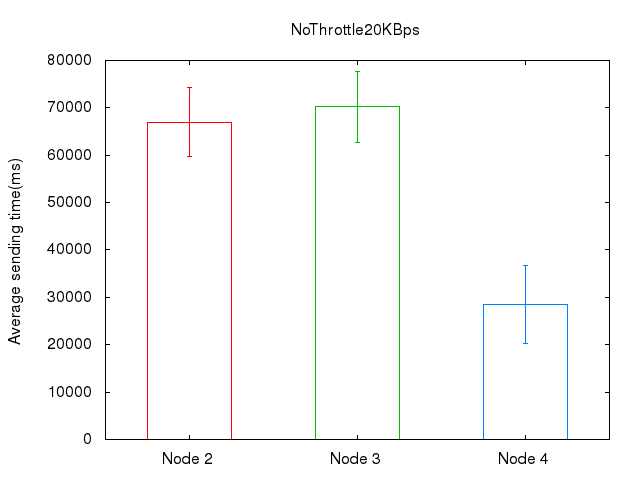
\includegraphics[scale=0.5]{NoThrottle20KBps_time}
		\caption{Time graph, no throttle mediator and bandwidth of 20kBps} 
		\label{figure:results:NoThrottle20KBps_time}
	\end{figure}
	
	As we expected without our throttle mediator, the time taken to receive messages back at the client is increased on all bandwidths where the bandwidth is below a certain threshold. Where the bandwidth is large enough, i.e. 40kBps, the time is comparable to our other tests because the bandwidth is more than large enough.
	
	
	The trend is also clear when it comes to successful messages, without our throttle mediator more messages arrive even on lower bandwidths.
	
	What is really interesting is that if we compare with a timeout of 100 000 our throttle mediator actually manages to get more high priority messages successfully back, across the board.
	
	\begin{figure}[H]
		\centering
		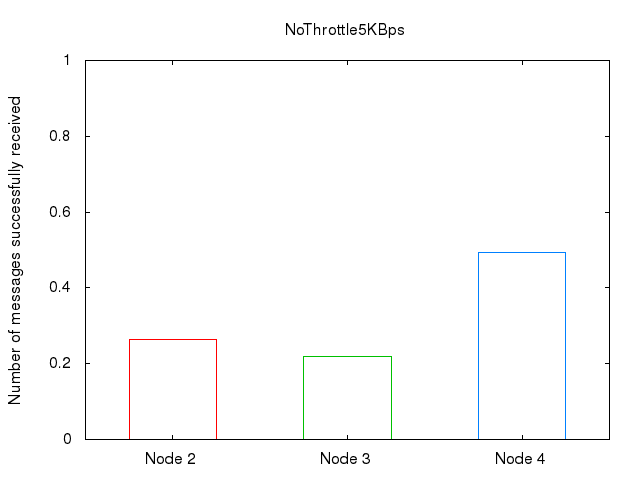
\includegraphics[scale=0.5]{NoThrottle5KBps_messages}
		\caption{Time graph, no throttle mediator and bandwidth of 5kBps} 
		\label{figure:results:NoThrottle5KBps_messages}
	\end{figure}
